\documentclass{standalone}
\usepackage{mathtools}
\usepackage{pgfplots}
\pgfplotsset{compat=1.17}
\begin{document}
	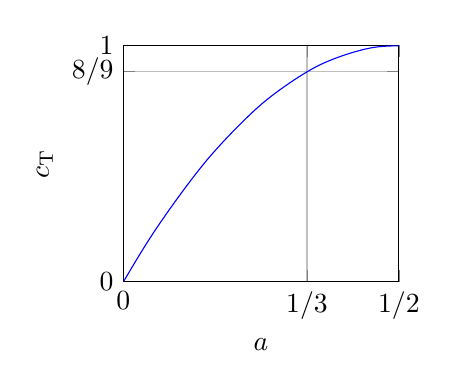
\begin{tikzpicture}
\begin{axis}[x=7cm,y=3cm,grid=major, xmin=0, xmax=0.5, ymin=0, ymax=1, xlabel=$a$, 
ylabel=$c_{\textnormal{T}}$,
ytick={0,8/9,1},
xtick={0,1/3,0.5},
yticklabels={0,8/9,1},
xticklabels={0,1/3,1/2}
]
\plot[blue] plot[samples=100, smooth] expression{4*x*(1- x)};
\end{axis}	
\end{tikzpicture}
\end{document}